% \begin{wrapfigure}{O}{0.5\textwidth}
\begin{figure}
  % \vspace{-30pt}
  \centering

  \begin{subfigure}[t]{0.49\textwidth}
    \hspace{-20pt}
  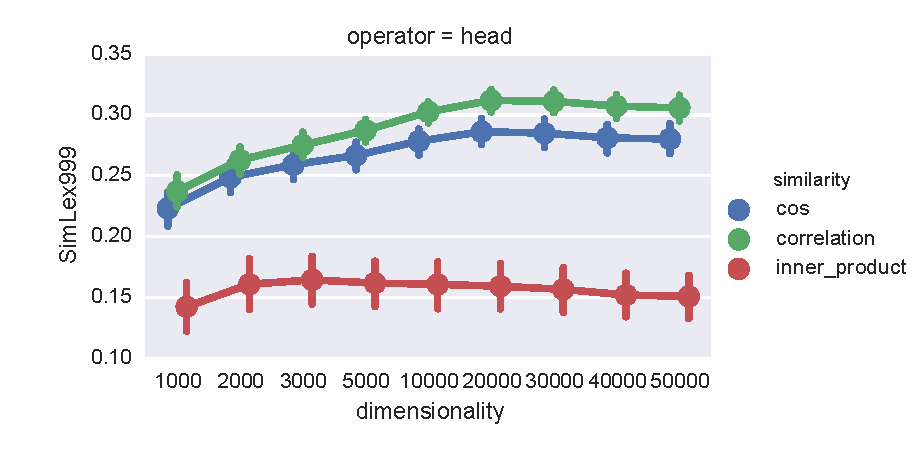
\includegraphics[width=1.1\textwidth]{supplement/figures/SimLex999-interaction-similarity}

  \caption{Similarity measure}
  \label{fig:SimLex999-similarity}

  \end{subfigure}
  \begin{subfigure}[t]{0.49\textwidth}

  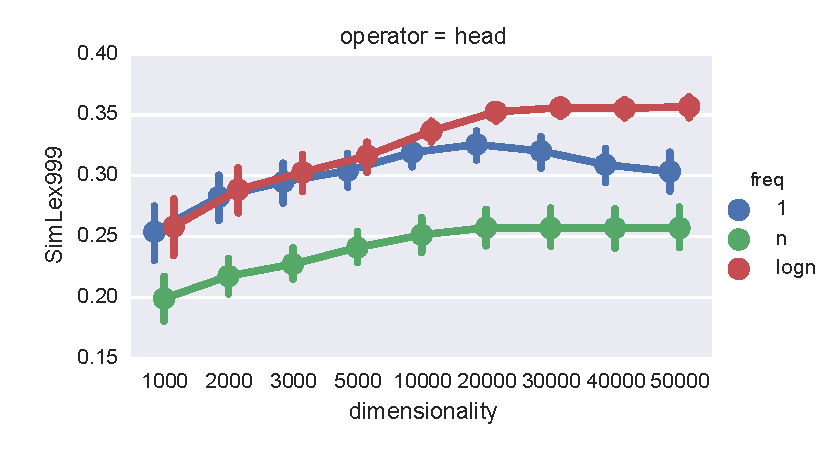
\includegraphics[width=\textwidth]{supplement/figures/SimLex999-interaction-freq}

  \caption{\texttt{freq}}
  \label{fig:SimLex999-freq}

  \end{subfigure}


  \begin{subfigure}[t]{0.49\textwidth}
  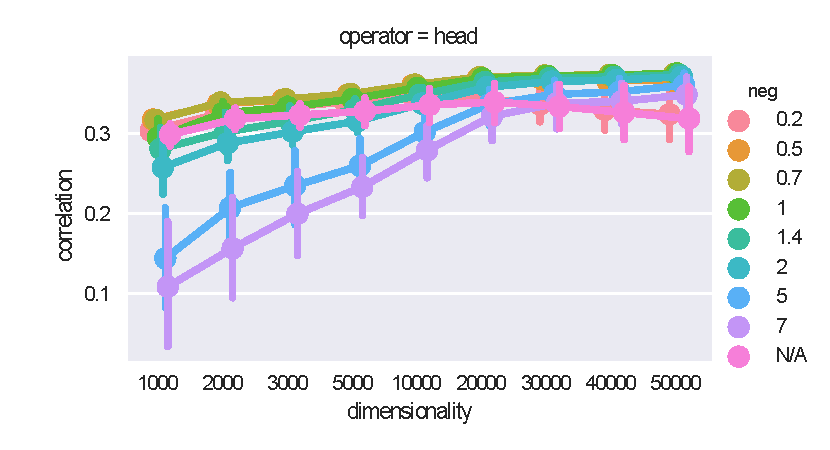
\includegraphics[width=\textwidth]{supplement/figures/SimLex999-interaction-neg}

  \caption{\texttt{neg}}
  \label{fig:SimLex999-neg}
  \end{subfigure}
  \begin{subfigure}[t]{0.49\textwidth}
  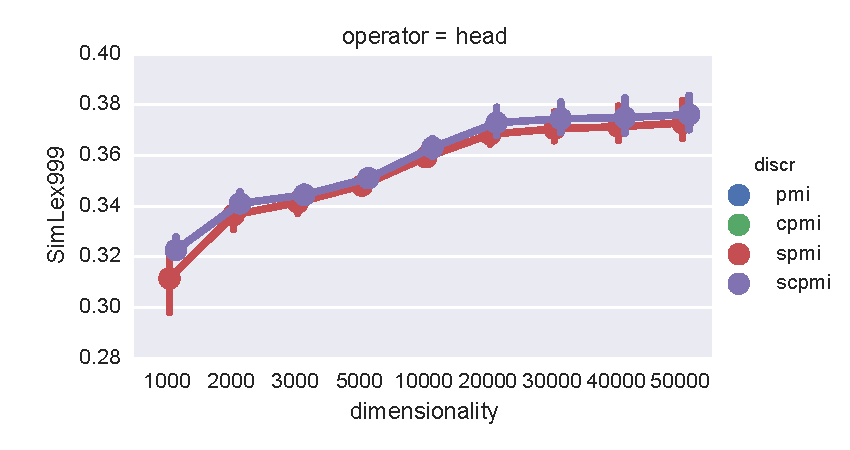
\includegraphics[width=\textwidth]{supplement/figures/SimLex999-interaction-discr}

  \caption{\texttt{discr}}
  \label{fig:SimLex999-discr}
  \end{subfigure}
  
  \caption[SimLex-999 influence of the similarity measure, \texttt{freq}, \texttt{neg} and \texttt{discr}]{SimLex-999 influence of the similarity measure, \texttt{freq}, \texttt{neg} and \texttt{discr}. For the values of minimal required difference for significance (MRDS) refer to Table~\ref{tab:mrds}.}
\end{figure}
